\subsection{Light-Curve Morphology} \label{sec:light-curve-morphology}

Transit photometry observes the flux from stars, searching for periodic decreases in brightness caused by a planet crossing the stellar disk \citep{Exoplanet_Detection_Methods}. This method has become the most successful approach for exoplanet detection, with over 4300 confirmed planets discovered through transits \citep{Num_Transit_Exoplanets_Discovered}. Since transit observations naturally represent stellar brightness as a function of time, a CNN can learn their depth, duration, and shape to make informed estimates of the origin of the data. An example of a Kepler transit light curve is shown in Figure~\ref{fig:example_transit_&_EB}.

\begin{align}
    \delta F \approx \left(\frac{R_p}{R_*}\right)^2 \label{eq:flux_depth}
\end{align}


Astronomers analyse many features in transit light curves which describe key parameters of the exoplanet system. The depth of the transit provides an estimate of the planet-to-star radius ratio, as shown in Equation~\ref{eq:flux_depth} \citep{2010exop.book...55W, 2003ApJ...585.1038S}. Here $\delta F$ is the change in normalized flux caused by the transit dip, while $R_p$ and $R_*$ represent the radii of the exoplanet and host star, respectively. As the ratio of radii between a planet and star is relatively small, planetary transits usually produce shallow decreases in flux. In eclipsing binary systems, the occulting body is another star, so the radius ratio is generally larger and the resulting eclipse depth is often but not always greater than that of a planetary transit.

\begin{figure}[h]
    \centering
    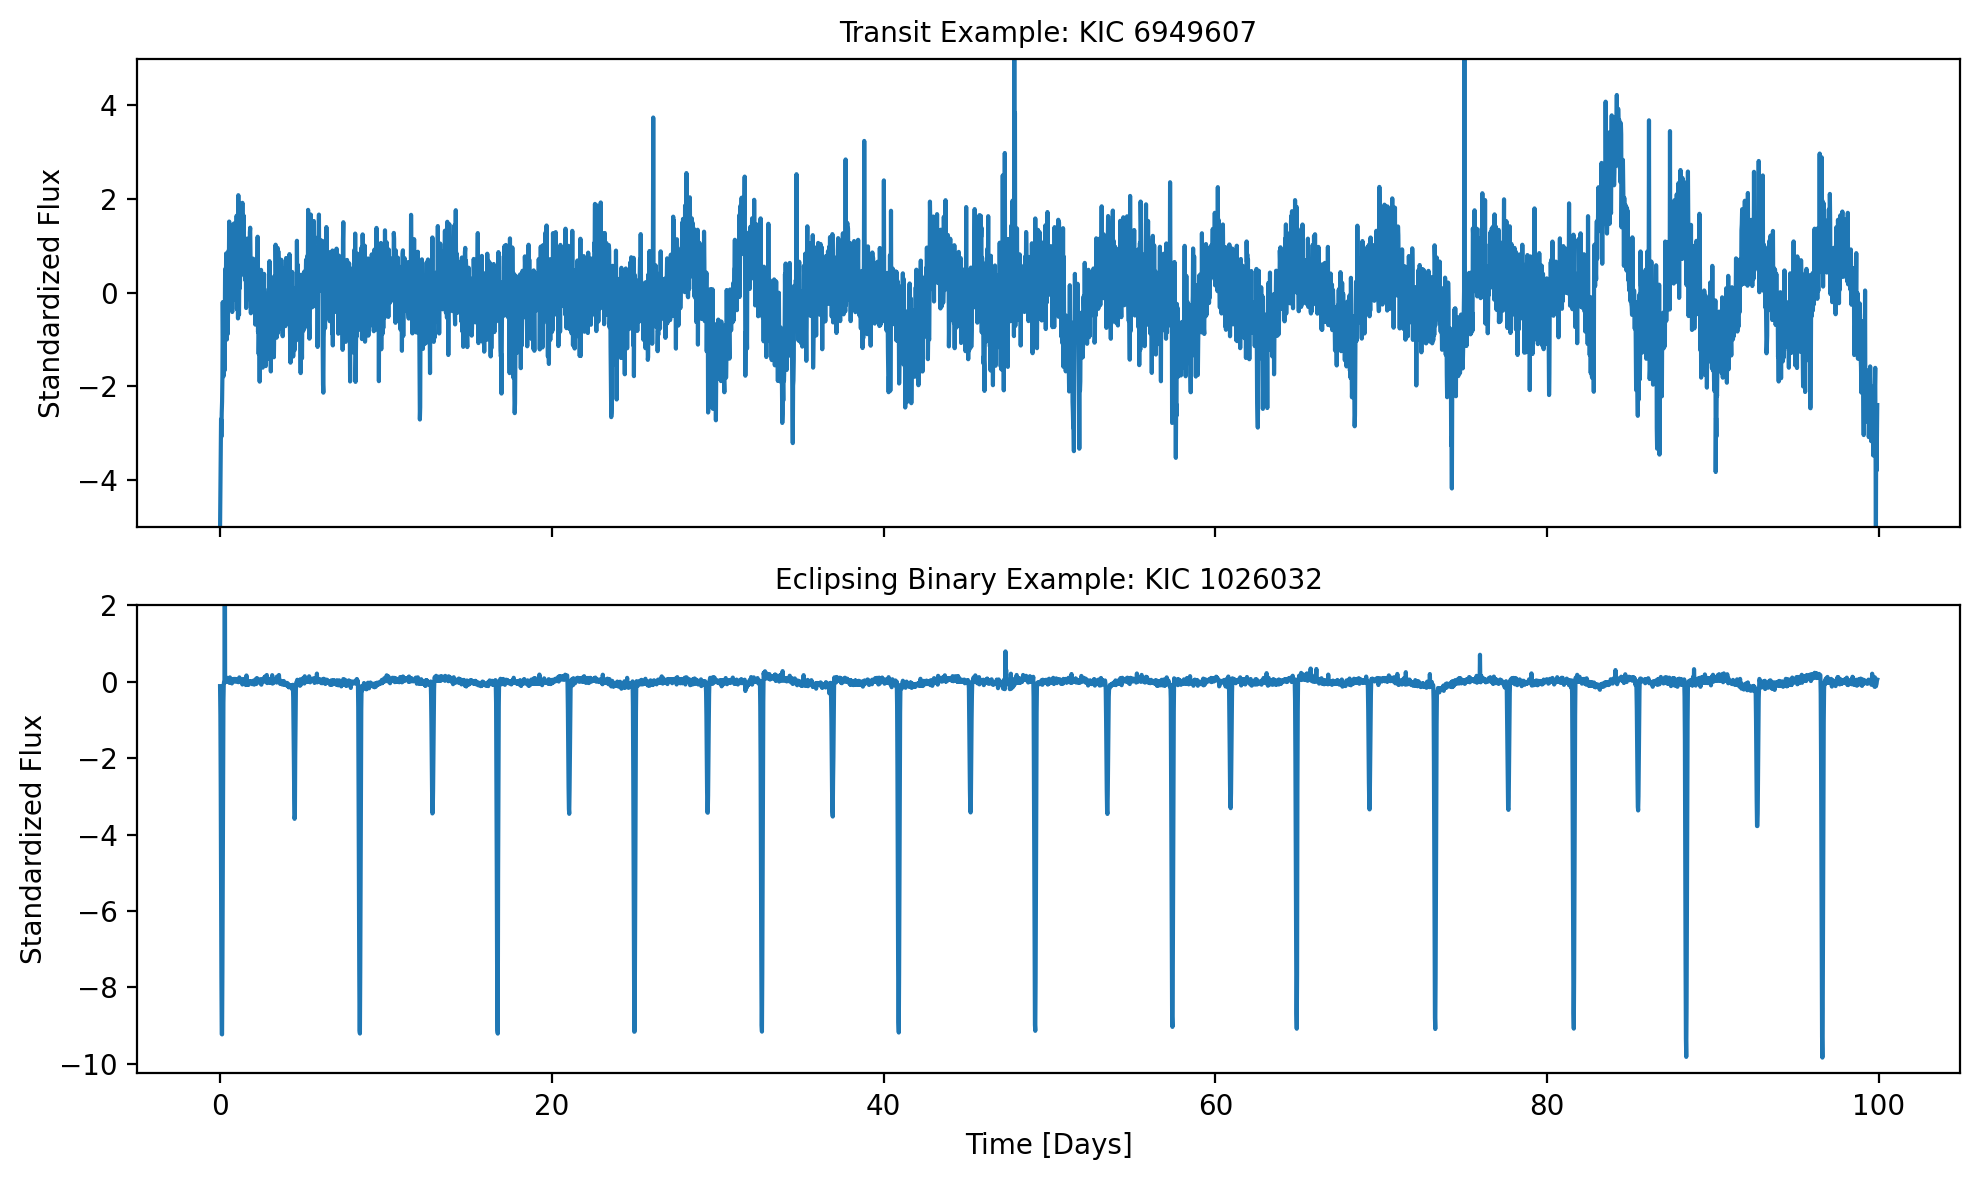
\includegraphics[width=0.99\linewidth]{figures/images/lightcurve_examples.png}
    \caption{Examples of the one-dimensional Kepler light curves used in the model training done in this paper. The plots show a 100-day chunk of KIC 6949607 and 1026032, the light curves of stars hosting a confirmed transiting exoplanet and confirmed eclipsing binary respectively. The model looks for features such as the dips and their duration and shape to classify the data as a transiting light curve. It can be seen how the transit example shows repetitive dips of relatively same depth while the eclipsing binary has a clear different in the two eclipses. The eclipsing-binary instance shows more pronounced dips in the standardized light curve, with the eclipse events extending further below the standardized baseline.}
    \label{fig:example_transit_&_EB}
\end{figure}

Transit shape also contains useful information. The ingress and egress are the times when the planet begins and ends its passage across the stellar disk, while the duration represents the total time spent between ingress and egress \citep{2010exop.book...55W}. Transiting exoplanets usually produce rounded, U-shaped dips, whereas eclipsing binaries can produce sharper V-shaped features that may resemble planetary-like signals \citep{2010exop.book...55W}. It is important to note that transits may also produce sharper V-like dips in the case of a grazing transit, where the planet does not fully pass across the stellar disk. Similarly, eclipsing binaries can produce more U-shaped eclipses depending on the geometry of the system \citep{2017MNRAS.465.2634A}. Thus, the shape is a useful tool for classification but is better combined with other factors for final predictions.